\documentclass{llncs}
\usepackage{tabu}
\usepackage{graphicx}
\usepackage[utf8]{inputenc}

\begin{document}

\title{EM Side-Channel Analysis of ECC Scalar Multiplication}
\author{Sebastian Verschoor, Alvin Cai Kunming}
\institute{Technische Universiteit Eindhoven, Eindhoven, The Netherlands}
\maketitle
%
\begin{abstract}
The aim of the project is to successfully run an electromagnetic side channel
attack on the Lim-Lee ECC scalar multiplication algorithm implemented on a
smart card.  \end{abstract} 
%
\section{Introduction}

The electric current that flows through a conductor induces Electromagnetic
(EM) emanations which can be used for side channel analysis. The advantage of
this technique is that it (a) allows the measurement of local EM radiations
from selected points on the chip \cite{gandolfi2001} and (b) attacks can be
mounted from a distance of several feet away \cite{kenworthy2012} e.g. against
mobile devices. EM measurements can potentially bypass any hardware
countermeasures that operates only on the power consumption of the entire chip.

In this paper, we attempt a practical attack on a smartcard performing ECC
scalar multiplication using EM analysis. This attack targets the Lim-Lee scalar
multiplication algorithm on Riscure's training card 8. In this report, we will
not go into details of the Lim-Lee algorithm and associated attack, but will
focus instead on the EM aspects which can be generalised to any scalar
multiplication algorithm.

\section{Methodology and Practical Results}

In our attack, we focus on the fact that EM provides us with a higher spatial
resolution. We first try to identify the specific location where cryptographic
operations are carried out on the smartcard. Then, we can position the EM probe
very close to this region so as to increase the chances of capturing
data-dependent signals. The EM traces we obtained were very noisy and required
signal processing to reduce noise to levels at which the data dependencies are
revealed. The final step of the attack is to perform a simple side channel
analysis to recover the secret key bits.

\begin{figure}
    \centering
    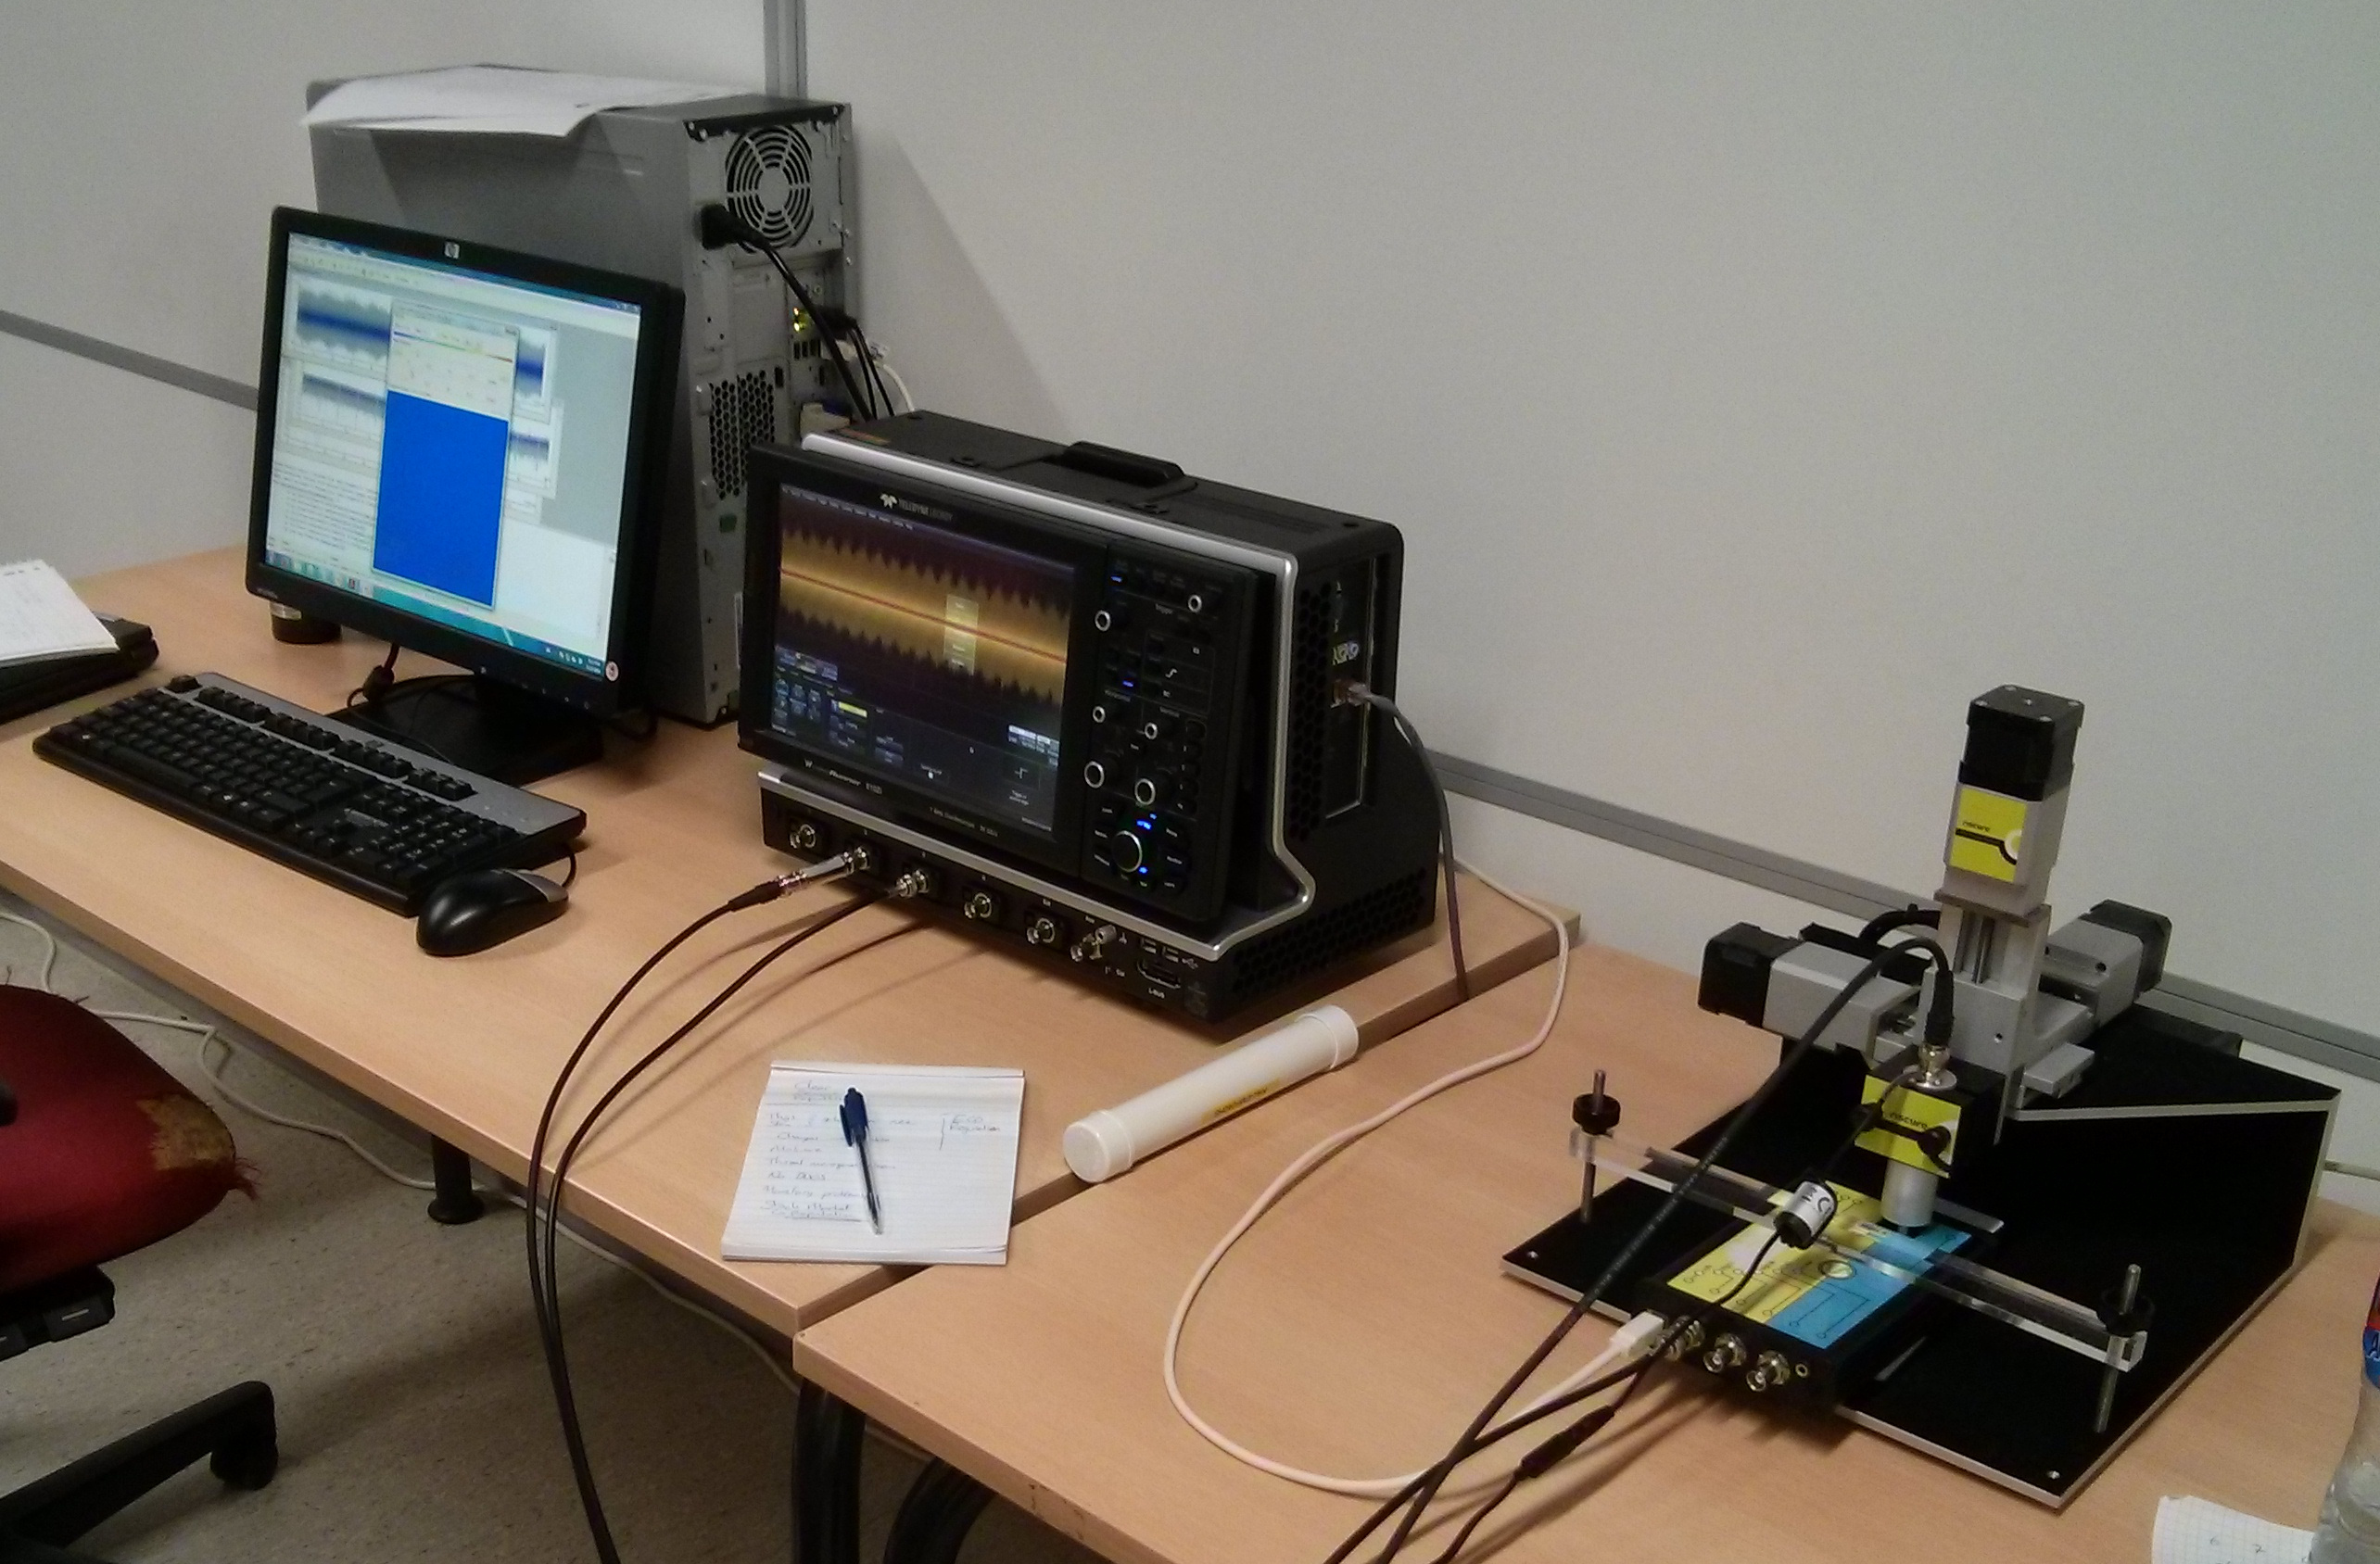
\includegraphics[width=\textwidth]{img/IMG_20140523_171003}
    \caption[]{Attack setup}
    \label{fig:setup}
\end{figure}

Figure \ref{fig:setup} shows the computer on the left, which is connected to
the oscilloscope in the center and to the smartcard reader on the right. The
computer stores both the data coming from the reader and the signal coming from
the oscilloscope. The oscilloscope pre-processes the data coming from the EM
probe and is connected to the trigger of the reader, so that it can start
measuring as soon as the trigger sends the required signal.

\begin{figure}
    \centering
    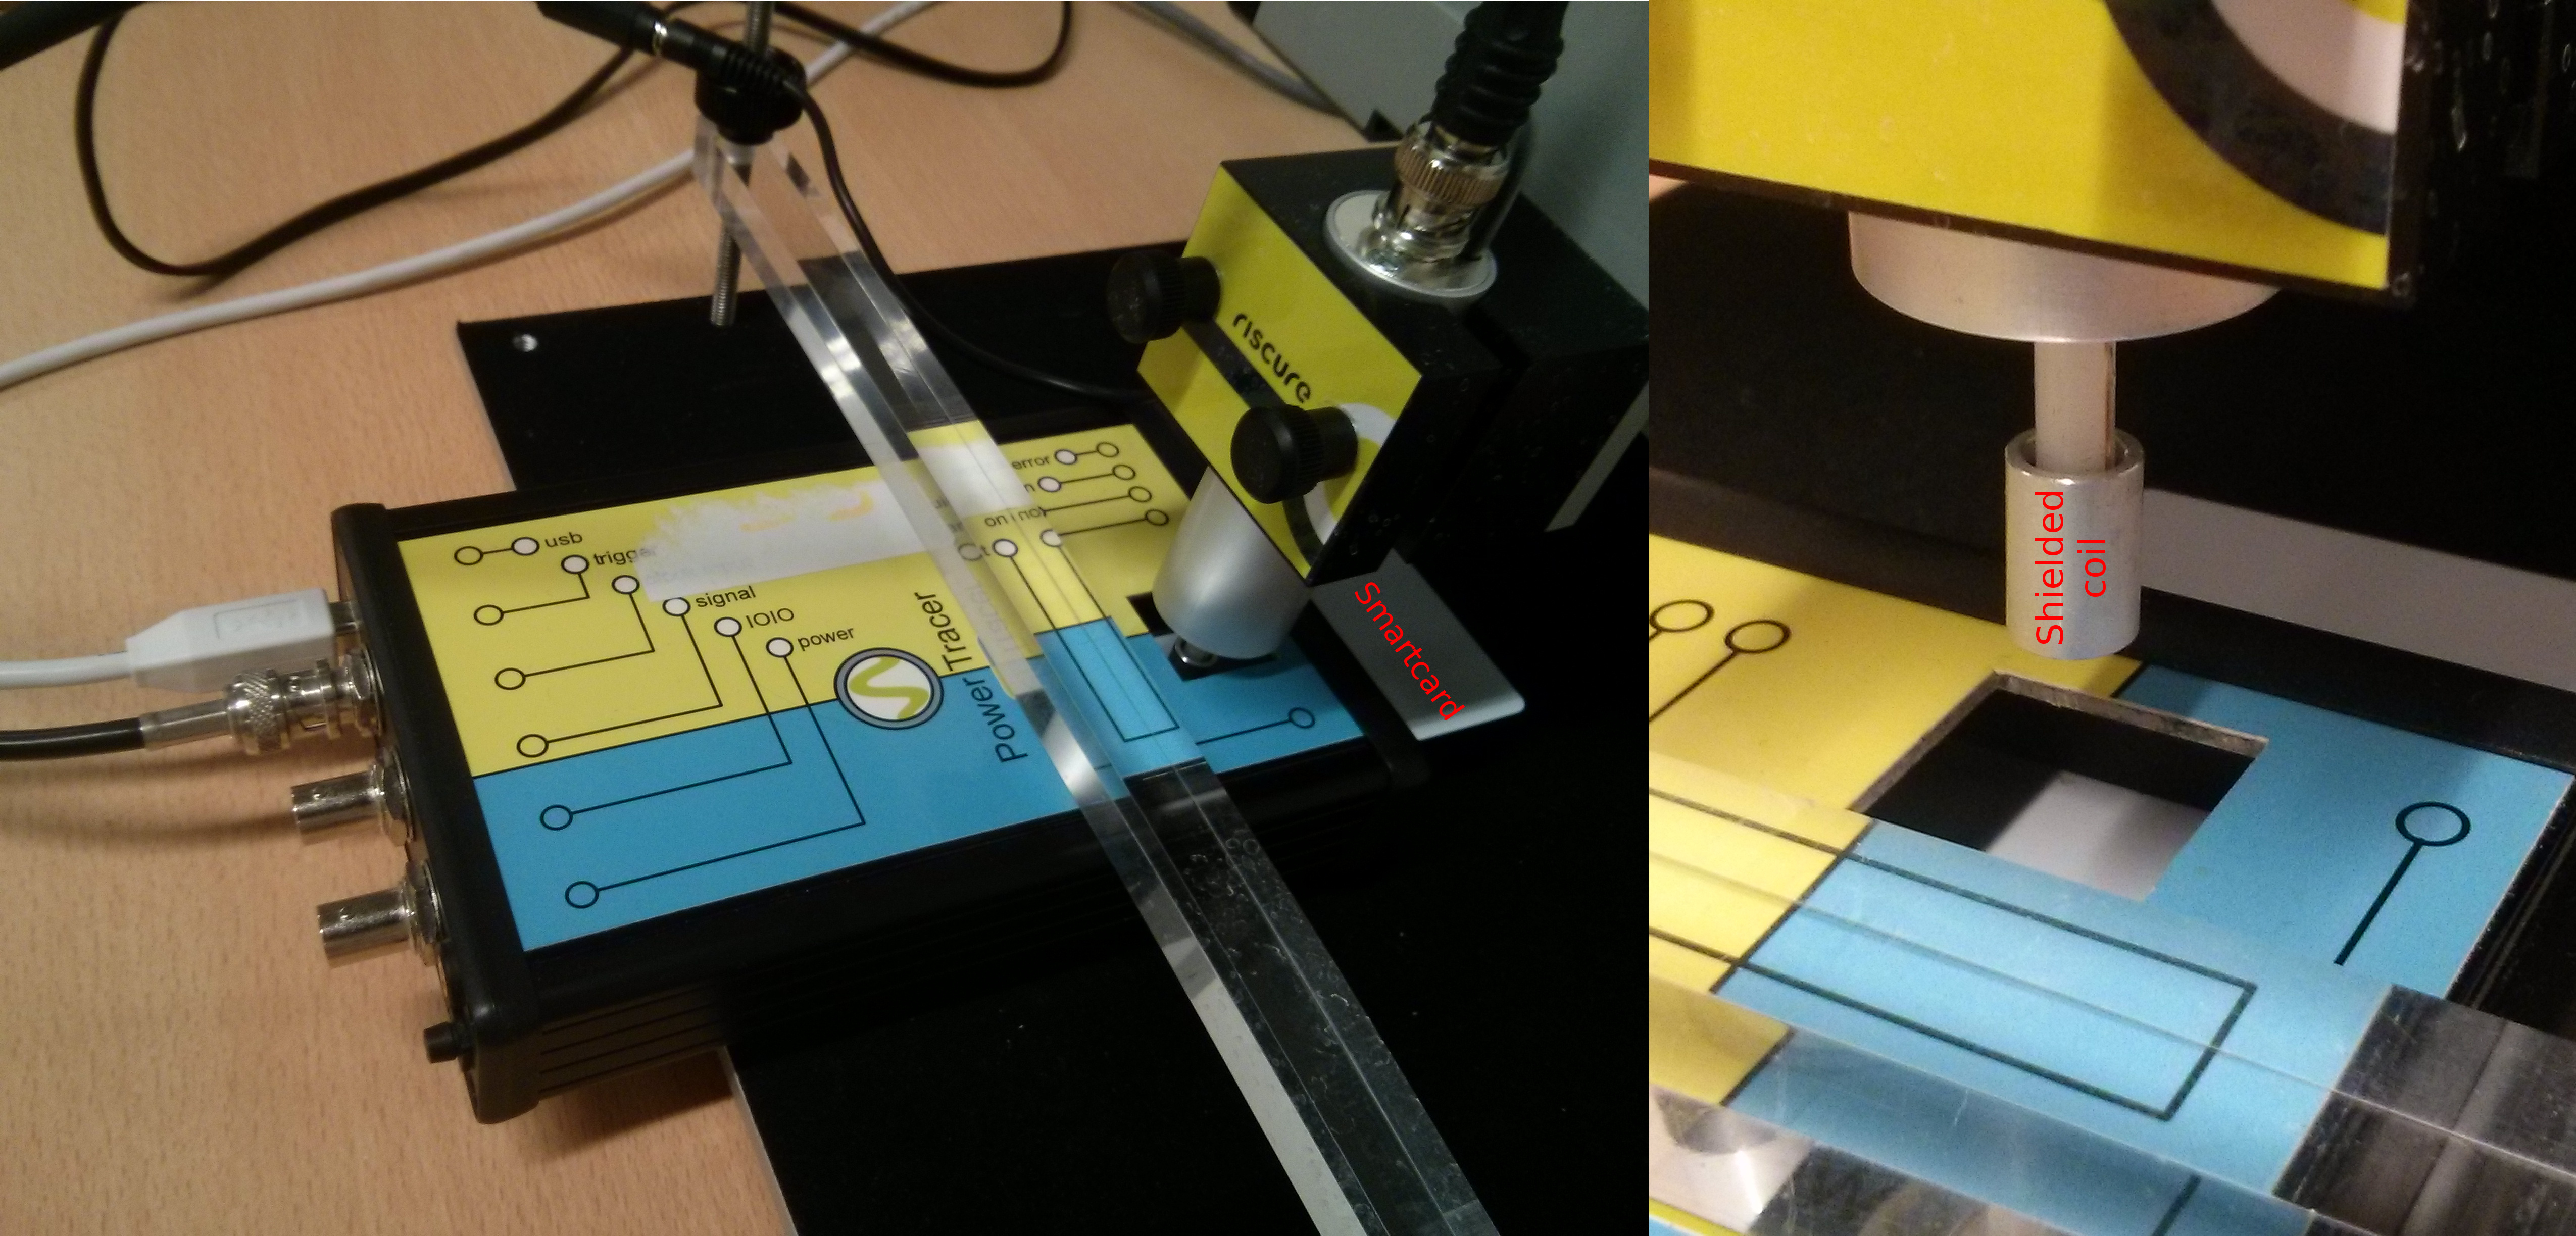
\includegraphics[width=\textwidth]{img/setup_probe}
    \caption[]{Attack setup: reader + probe}
    \label{fig:setupreader}
\end{figure}

Figure \ref{fig:setupreader} shows the smartcard reader (which can also act as
a power tracer), the EM probe (the metallic cylinder) and the smartcard. This
contraption is held in place by the positioning device, which can position the
probe on the card very accurately. This probe works on the simple principle
that changes in the magnetic field in the coil induce electricity on the coil
wire, which can be measured. % Alvin please correct me if I am wrong here...
By placing the coil very close to the smartcard chip, the probe can measure the
magnetic field that is generated by the electricity flowing through the chips
wires.

\subsection{Spatial Positioning}

The first step of the attack is to find the relevant part of the chip for doing
the cryptanalysis, so that we can place the coil directly above it for our
measurements. On the card we attacked, this corresponded with finding the
cryptographic chip that executed the multiplication algorithm. The below steps
suggest a straightforward course of action, but reality was more a trial and
error process.

To find the cryptographic chip, we challenged the card while measuring at
different points on the chip. This was automated with the Inspector software,
so that we captured a trace for each (x,y) coordinate in a 9x9 grid. We
inspected the spectogram\footnote{a plot of time on the vertical axis,
frequency on the horizontal axis and amplitude as the color intensity for each
coordinate} for several traces. Besides the distinct vertical bars at 4MHz (the
inputted clock signal), in some traces we observed high intensity at 30.8MHz.
We suspect that this is the frequency at which the cryptographic chip operates.
This hypothesis is further strengthened by the observation that there is a
brief period at the beginning of the trace in which this frequency is absent (a
gap in the vertical line in the spectogram).

A small side note here is in order. Our first hypothesis was that the
cryptographic chip was running at 38.4MHz, because this frequency also showed a
high intensity, except for the same brief period in the beginning. At closer
inspection we observed that we could see high intensity at several harmonics of
about 7.7MHz, with the highest peaks at 30.8MHz and 38.4MHz. The tutorial
suggested that the cryptographic chip was in fact operating at 30.8MHz, so we
have no plausible explanation for this observation.

From the traces we computed a Spectral Intensity diagram, which displays the
overall spectral intensity for each of the traces from the 9x9 grid. By
filtering out any frequency below 30.2MHz and 31.3MHz, we could identify a
region in the lower right corner of the chip that showed much activity at the
required frequency, so this was probably the location of the cryptographic
chip.

To find a region from which we could observe good measurements, we again took
measurements in a 9x9 grid, but now zoomed in on a smaller region, thereby
increasing the spatial resolution. We repeated the process once more to zoom in
further (although with a slightly smaller amount of grid points). It turned out
the traces that did not have the highest spectral intensity, but just slightly
below gave us the best signal for extracting confidential data.

\subsection{Signal Processing}

The first step in the signal processing was to isolate the information bearing signal. The most straightforward step was hence to remove the 4MHz signal and its harmonics that arise from the main processor. The 30.8 GHz signal we are interested in is preserved as shown in Figure \ref{figure:harmonics_removal}.

    \begin{figure*}
      \centering
      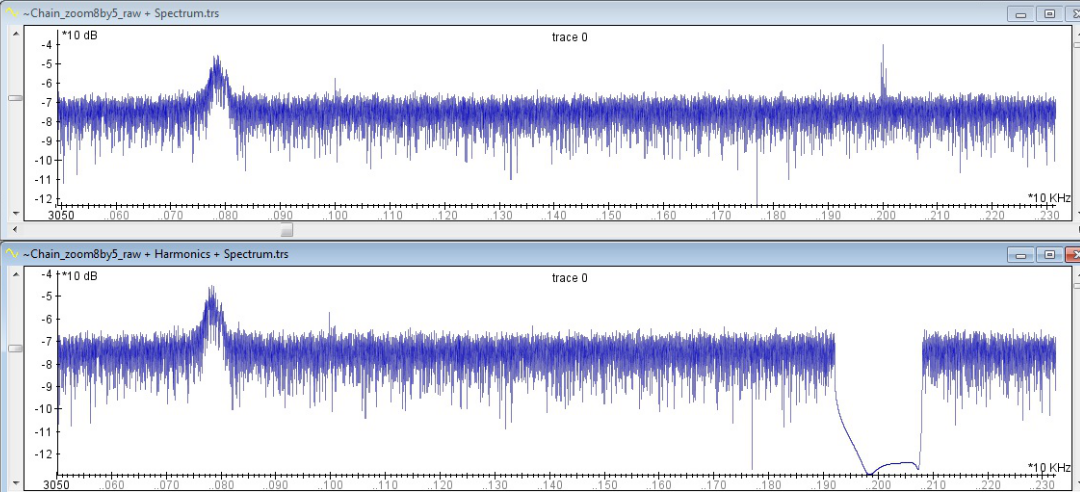
\includegraphics[scale=0.3]{img/harmonics_removal.png}
      \caption{\label{figure:harmonics_removal}Removal of 4GHz harmonics.}
    \end{figure*}  

The EM signal was sampled at a very high frequency (250 Mhz to 1 GHz), and fluctuates frequently between positive and negative values. To better analyse the signal, we try to obtain the absolute value of the signal envelope by using the ``Sync Resample" module which  resamples the original signal at a 30.8 MHz sample rate. Thereafter, we perform low pass filtering. 

These three steps were sufficient to produce a sufficiently clear signal for simple side channel analysis. In the Lim-Lee algorithm, a single scalar multiplication has many rounds. At the beginning of each round, we observe a distinct pattern of 5 or 7 bumps as shown in Figure \ref{figure:pattern}. Here, 5 bumps indicate a 0-bit and 7 bumps indicates a 1-bit value of the nonces used in Lim-Lee. Sufficient nonce values can be obtained across approximately 50 traces (using different input points) to recreate the secret ECC scalar.

Although these three signal processing steps were sufficient, we could additionally have averaged multiple EM traces (using the same  input Point) to produce an even clearer signal, for each of the required 50 traces.

    \begin{figure*}
      \centering
      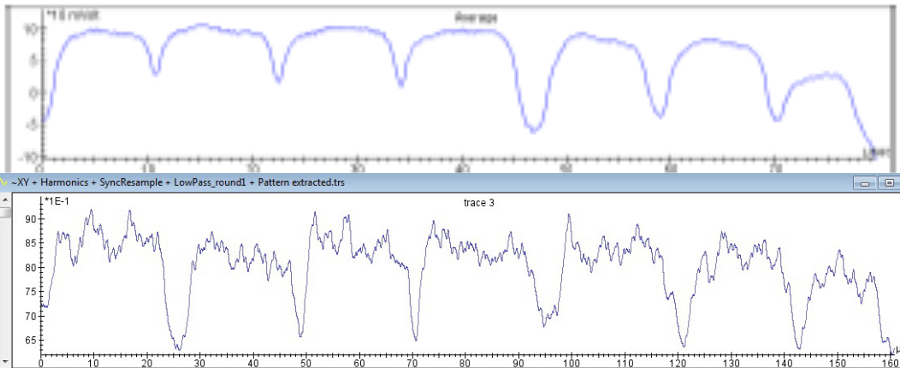
\includegraphics[scale=0.3]{img/pattern.png}
      \caption{\label{figure:pattern}The upper image was obtained from an unfiltered power trace. The lower image was our actual EM measurements after signal processing.}
    \end{figure*}  






\subsection{Simple Side Channel Analysis}
\begin{enumerate}
  \item just provide a brief description as anyway we did not do this completely. 
  \item I think its more interesting to talk about how we can perform a proper attack given the limitations (i.e. can only measure short sections each time.)
  \item \ldots
\end{enumerate}





\section{Conclusion}

Our findings show that EM works as a side channel attack method, as we did
extract one bit of information leading to the extraction of the secret key.
With enough time on our hands, we could definitely implement a complete (and
possibly fully automated) attack to extract the key from the device. The
problem with the required high sampling rate reduces the amount of data we can
extract per measured trace. Since each measurement takes quite some time, the
attack would not be very fast, especially compared to a more common SPA attack
that extracts more bits per measurement.

Our results can hardly be generalized to different scenario's, because our
attack was limited to a single training card which contained a separate
cryptographic chip. Literature suggests that EM attacks can work without making
contact with the card. However, our findings show that the method is highly
susceptible to spatial errors: the strength of the desired signal seems to drop 
significantly when we shift a few millimeters away from the cryptographic chip.

It might be interesting to conduct further experiments on the efficiacy of signal recovery 
at different locations and distance. This could provide insights into the factors which 
impact distance based EM attacks.

% Add entries in the bibliography that aren't cited:
% \nocite{gandolfi2001}
% \nocite{kenworthy2012}

\bibliographystyle{splncs03}
\bibliography{literature}
% \begin{thebibliography}{99}
% 
% \bibitem{Gandolfi}
% Gandolfi, Karine, Christophe Mourtel, and Francis Olivier. "Electromagnetic analysis: Concrete results." Cryptographic Hardware and Embedded Systems—CHES 2001. Springer Berlin Heidelberg, 2001.
% 
% \bibitem{cri}
% Gary Kenworthy and Pankaj Rohatgi. "Mobile Device Security: The case for side channel resistance." Cryptography Research Inc, 2012.
% 
% 
% \end{thebibliography}
\end{document}
